\section{Engineering: the toolkit, the bug catalog, and the ladder}\label{sec:engineering}

\mkey{the toolkit}The entry barrier to this field has fallen steadily --- a solo engineer can now reproduce Deep-CFR-class results --- but the tools have sharply different roles, and the sweep behind this survey found the community's hard-won bug list scattered across tutorials, ablations, and GitHub issues. Both are collected here.

\begin{center}
\footnotesize
\begin{tabular}{@{}lp{2.45in}p{1.5in}@{}}
\toprule
Tool & Role in this project & Trust level \\
\midrule
OpenSpiel~\cite{openspiel} & the \emph{referee}: reference CFR + exact exploitability on Kuhn/Leduc; verify your numbers against it & tabular code: high; its Deep CFR: has open bug reports \\
PokerRL~\cite{pokerrl} & the \emph{architecture reference}: Deep CFR/SD-CFR + a graded BR$\to$LBR$\to$RL-BR evaluation ladder, by SD-CFR's author & read and port from; frozen on PyTorch 0.4 --- do not depend on \\
PokerKit~\cite{pokerkit} & the \emph{rules oracle}: variant poker (draws, splits) as configuration, 99\% test coverage; unit-test the custom engine against it & good; pure-Python speed, so not the inner loop \\
RLCard~\cite{rlcard} & quick sandbox, clean encoding patterns & fine for prototypes; weak equilibrium tooling \\
\bottomrule
\end{tabular}
\end{center}

\mnote{No library implements Drawmaha itself --- the split-pot draw engine is genuinely custom work; the tools above check it rather than replace it.}\textbf{Hand evaluation sits on the critical path}: every MCCFR terminal node needs \emph{two} evaluations (inner hand, outer hand), millions of times per run. The classic lineage solves it: all 5-card hands collapse to exactly 7{,}462 distinct strength classes (Cactus Kev), reachable by perfect-hash lookup in a handful of memory reads~\cite{cactuskev}; open C/C++ evaluators (OMPEval, PokerHandEvaluator with its Omaha mode) are $10$--$100\times$ faster than Python ones. Since Drawmaha hands are exactly five cards, the 5-card perfect hash fits natively; Ho's bit-packing (Section~\ref{sec:precedents}) makes the split-pot comparison one integer operation.

\subsection*{The bug catalog}

Five bugs account for most broken CFR implementations in the community record; all are \emph{silent} --- nothing crashes, the answer is just wrong:

\begin{center}
\footnotesize
\begin{tabular}{@{}p{1.85in}p{2.75in}@{}}
\toprule
The bug & The rule that prevents it \\
\midrule
Reach-probability swap & regrets weight by \emph{opponent+chance} reach; average-strategy accumulation weights by \emph{own} reach --- never the reverse (Section~\ref{sec:cfr}) \\
Querying the current strategy & every guarantee is about the \emph{average}; vanilla CFR's current strategy cycles forever (Fig.~\ref{fig:kuhn}) \\
Missing iteration weights & linear averaging means weighting by $t$ --- in tabular sums \emph{and} in Deep CFR's buffer samples \\
Missing sampling correction & outcome sampling must divide by the sample probability; external sampling needs no correction --- one reason to prefer it \\
FIFO instead of reservoir & Deep CFR's buffers must be uniform over \emph{all} iterations; recency-biased buffers break the average \\
\bottomrule
\end{tabular}
\end{center}

The antidote to all five is the same discipline: \hlight{regression-test against known values at every stage --- Kuhn's closed-form equilibrium and game value ($-1/18$), Leduc's sequence-form-LP value ($-0.085606\ldots$ for player 1), and OpenSpiel's exploitability curves reproduced iteration-for-iteration.} This paper's own Figure~\ref{fig:kuhn} pipeline was validated exactly this way (and Section~\ref{sec:evaluation} confessed the bug the check caught).

\subsection*{Compute reality, and the ladder that structures the build}

Figure~\ref{fig:compute} places the landmark systems on one axis, and it doubles as the argument for the project's scope: the tabular triumphs (Cepheus) and the search flagships (ReBeL) sit orders of magnitude beyond a solo budget, while Deep CFR's published recipe is single-GPU-class --- \emph{the} reason it is the chosen endgame. \mnote{Modal GPUs cover the Deep CFR phase if the laptop doesn't; nothing in the plan needs a cluster.}

\begin{figure}[t]
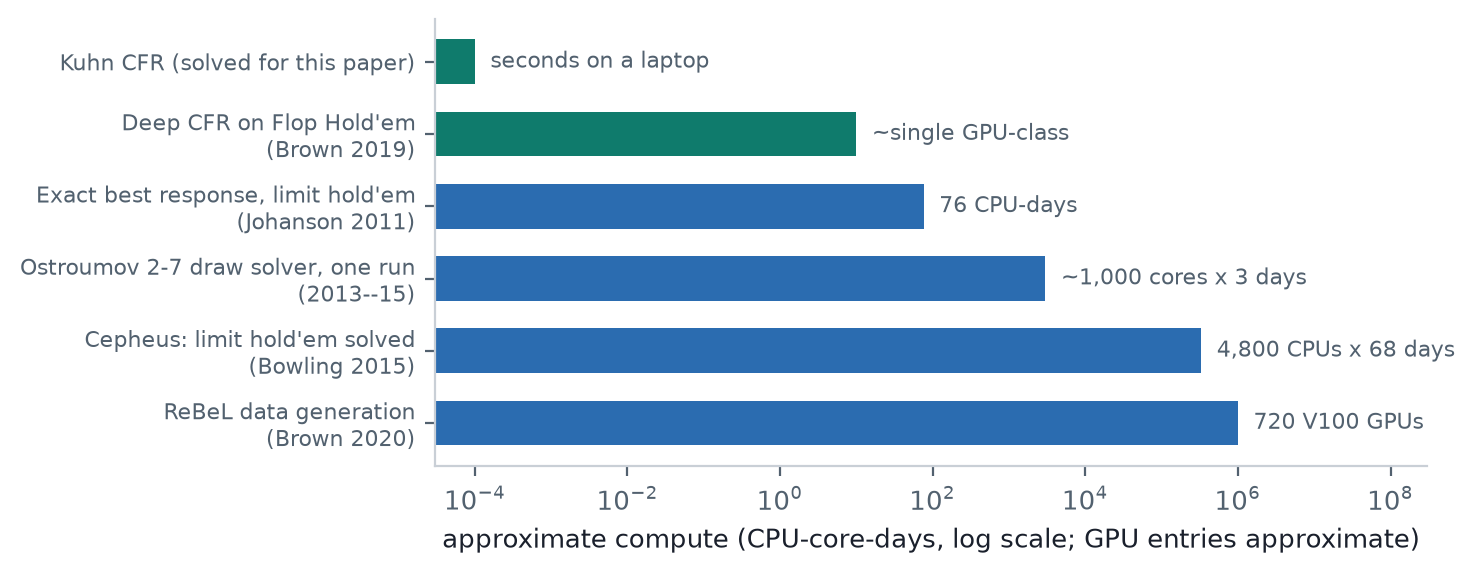
\includegraphics[width=\linewidth]{figures/compute.png}
\caption{Approximate compute of landmark systems, from reported hardware (log scale; order-of-magnitude estimates).}
\label{fig:compute}
\end{figure}

The build itself follows the field's standard validation practice --- prove each layer on a game with a known answer before adding the next --- instantiated for this project as Figure~\ref{fig:ladder}'s ladder. Its logic: Deep CFR has three separately-breakable layers (the CFR core, the Drawmaha rules engine, the networks); climbing one rung at a time means every failure has one suspect. The mini-drawmaha rung earns special emphasis: it is where all three Drawmaha-specific mechanisms (split pot, draw round, face-up draw-1) get proven while exact evaluation is still possible --- and it doubles later as tier 1 of the full evaluation (Section~\ref{sec:evaluation}).

\begin{figure}[t]
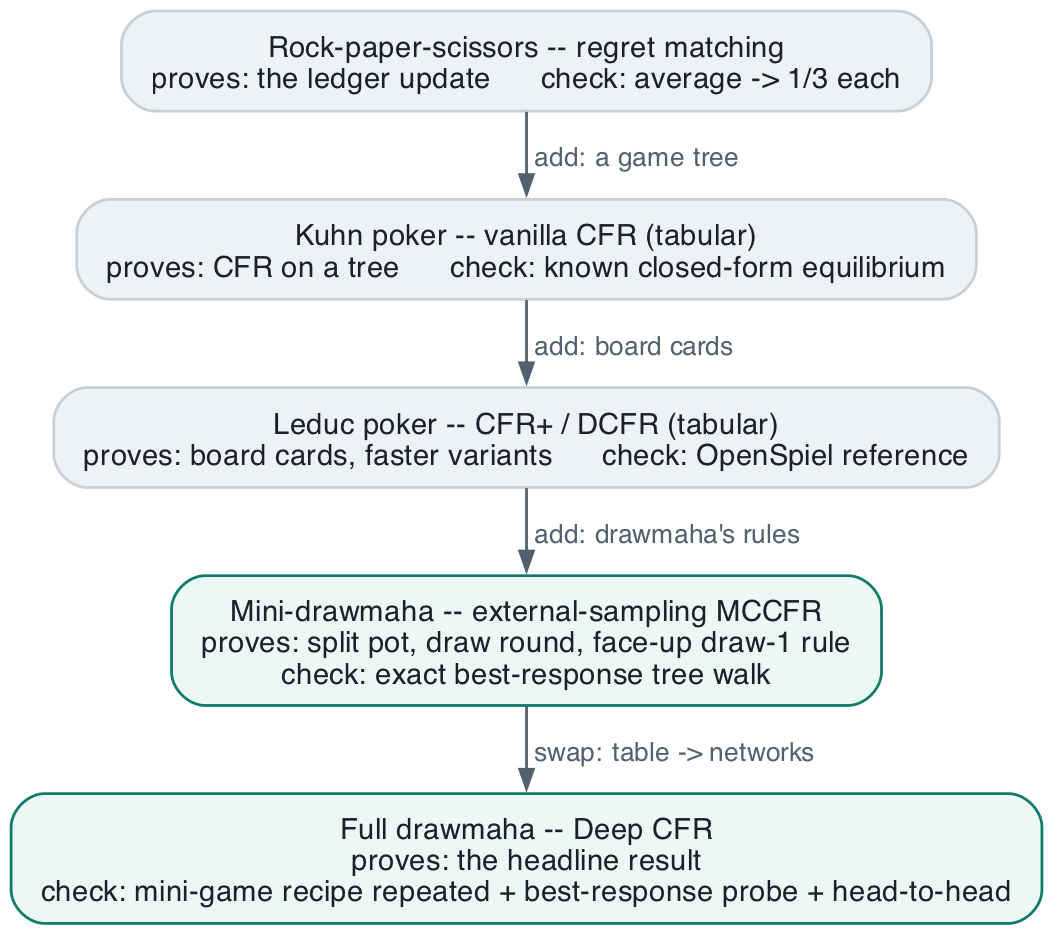
\includegraphics[width=\linewidth]{figures/ladder.png}
\caption{The project's validation ladder: one new layer per rung, a known answer at every rung.}
\label{fig:ladder}
\end{figure}
